\section{Complex LMS and Widely Linear Modelling}

\begin{enumerate}[label=\alph*), leftmargin=*]

%% a)
\item
%

A Wide Linear Moving Average order 1, WLMA(1), process $y(n)$ is generated, whose \texttt{real} and \texttt{imag} parts are provided in figure \ref{fig:4_1_a}.
As expected, the process is not circular, and we expect simple Complex Least Mean Squared (CLMS) algorithm to fail to model it.

The mean squared prediction error curve in figure \ref{fig:4_1_a} agrees with our assumption, though the Augemented Complex Least Mean Squared (ACLMS) algorithm
successfully learns the process parameters. In more detail, the ACLMS achieves an $MPSE = -300dB$ in steady-state, while CLMS saturates at $MPSE = 7.6$. This is
the consequence of the inability of the CLMS to adapt to non-circular signals, due to its limited capacity.

\begin{figure}[h]
    \centering
    \begin{subfigure}{0.49\textwidth}
        \centering
        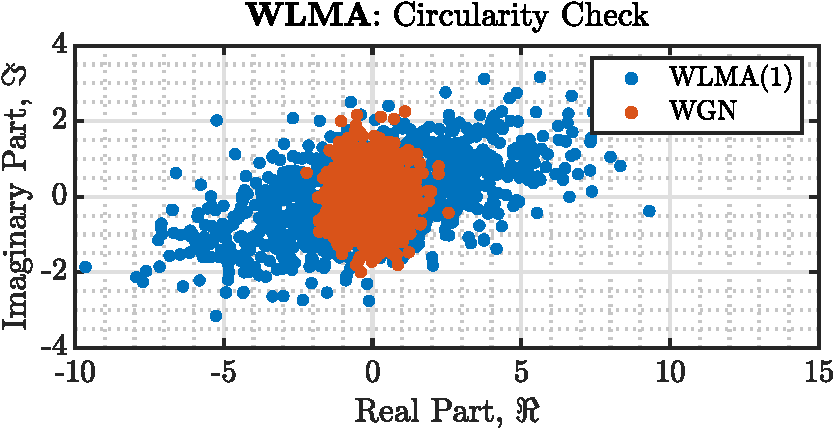
\includegraphics[height=1.5in]{report/widely-linear-filtering-and-adaptive-spectrum-estimation/complex-LMS-and-widely-linear-modelling/assets/a/comparison}
    \end{subfigure}
    ~
    \begin{subfigure}{0.49\textwidth}
        \centering
        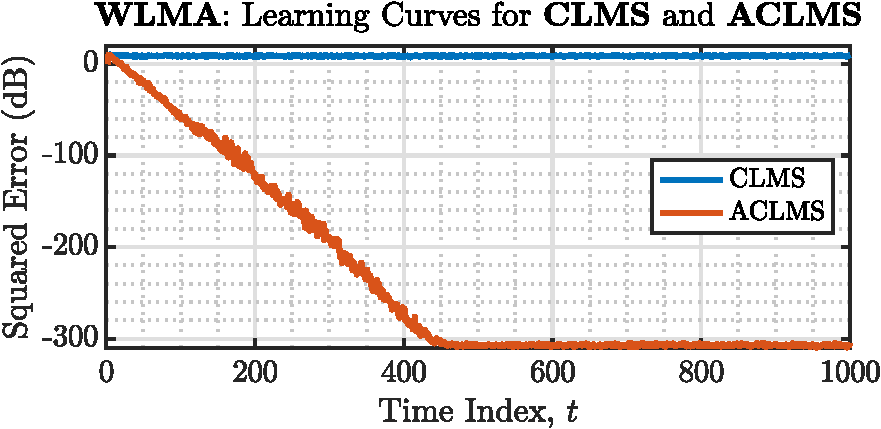
\includegraphics[height=1.5in]{report/widely-linear-filtering-and-adaptive-spectrum-estimation/complex-LMS-and-widely-linear-modelling/assets/a/learning_curves}
    \end{subfigure}
    \caption{CLMS vs ACLMS: non-circularity and (A)CLMS learning curves.}
    \label{fig:4_1_a}
\end{figure}

%% b)
\item
%

Figures \ref{fig:4_1_b_1}, \ref{fig:4_1_b_2}, \ref{fig:4_1_b_3} illustrate the circularity plots (\texttt{real}-\texttt{imag} scatter plots) along with the learning curves
of the ACLMS and CLMS algorithms for different model orders, on the \texttt{wind-dataset}.

Despite its non-obviously symmetric shape, the low regime wind data has lowest circularity coefficient, $\rho = 0.159$, while the medium and high regimes have
$\rho = 0.454$ and $\rho = 0.624$, repsectively. A complex-valued random variable is said to be circular if its probability distribution is not dependent on the angle, that is,
the distribution is rotationally invariant. In other words the variable’s probability distribution function should only depend on the Euclidean distance from the origin in the complex domain.
By definition, the higher the circularity coefficient, $\rho$, the less circular the data is.

Hence, as shown in the previous part, ACLMS algorithm outperforms CLMS on non-circular data. This is verified again on the \texttt{wind-dataset}, where the ACLMS has lower 
mean squared prediction error (MPSE) for any wind regime. More interesting is the fact that at high regime data, the least circular, the ACLMS has a larger margin in performance
($0.1 dB$). Lastly, we observe that the MPSE is minimised for small model orders, $M \in [3, 6]$, since over-modelling leads to over-fitting the noise and fail to generalise, despite
the excess degrees of freedom. For larger model order, $M > 10$, we observe that the ACLMS performs worse than the CLMS, due to its extra capacity (more parameters), which lead to
overfitting.

\begin{figure}[h]
    \centering
    \begin{subfigure}{0.49\textwidth}
        \centering
        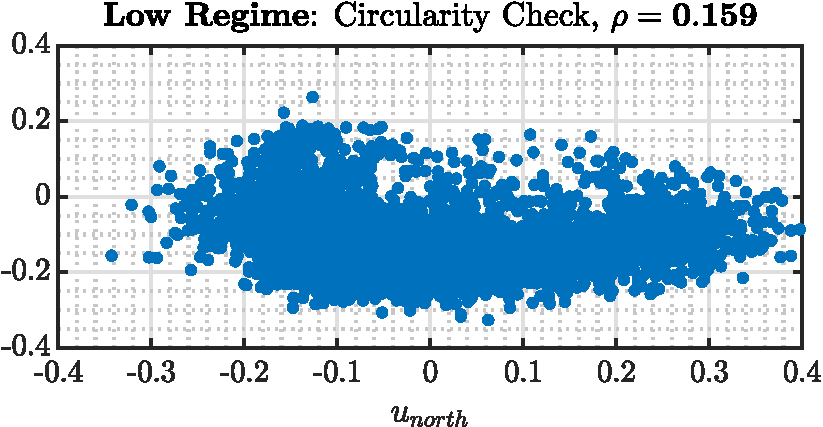
\includegraphics[height=1.5in]{report/widely-linear-filtering-and-adaptive-spectrum-estimation/complex-LMS-and-widely-linear-modelling/assets/b/circularity_1}
    \end{subfigure}
    ~
    \begin{subfigure}{0.49\textwidth}
        \centering
        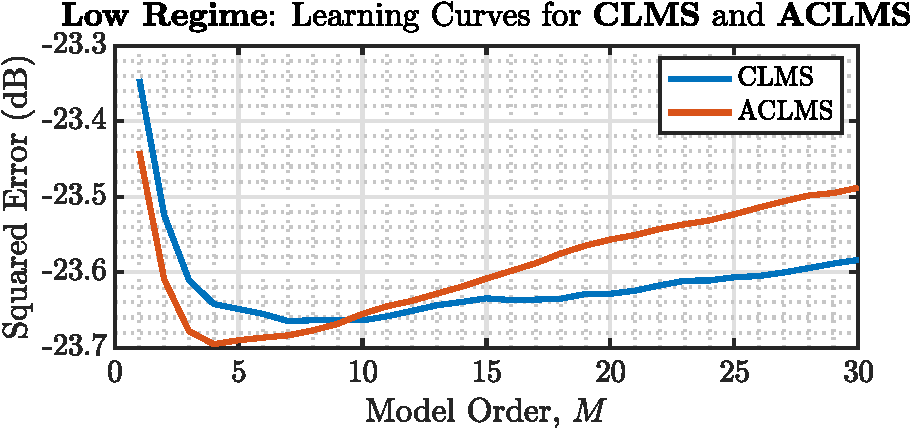
\includegraphics[height=1.5in]{report/widely-linear-filtering-and-adaptive-spectrum-estimation/complex-LMS-and-widely-linear-modelling/assets/b/learning_curves_1}
    \end{subfigure}
    \caption{Low Regime:circularity plot and (A)CLMS learning curves.}
    \label{fig:4_1_b_1}
\end{figure}

\begin{figure}[h]
    \centering
    \begin{subfigure}{0.49\textwidth}
        \centering
        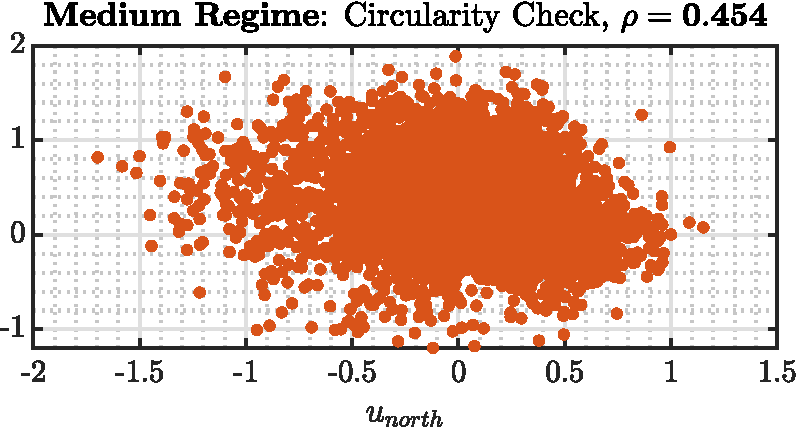
\includegraphics[height=1.5in]{report/widely-linear-filtering-and-adaptive-spectrum-estimation/complex-LMS-and-widely-linear-modelling/assets/b/circularity_2}
    \end{subfigure}
    ~
    \begin{subfigure}{0.49\textwidth}
        \centering
        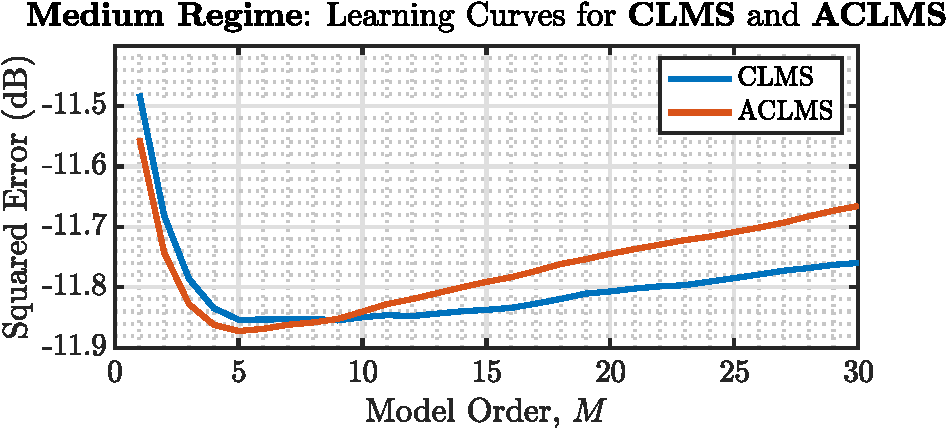
\includegraphics[height=1.5in]{report/widely-linear-filtering-and-adaptive-spectrum-estimation/complex-LMS-and-widely-linear-modelling/assets/b/learning_curves_2}
    \end{subfigure}
    \caption{Medium Regime:circularity plot and (A)CLMS learning curves.}
    \label{fig:4_1_b_2}
\end{figure}

\begin{figure}[h]
    \centering
    \begin{subfigure}{0.49\textwidth}
        \centering
        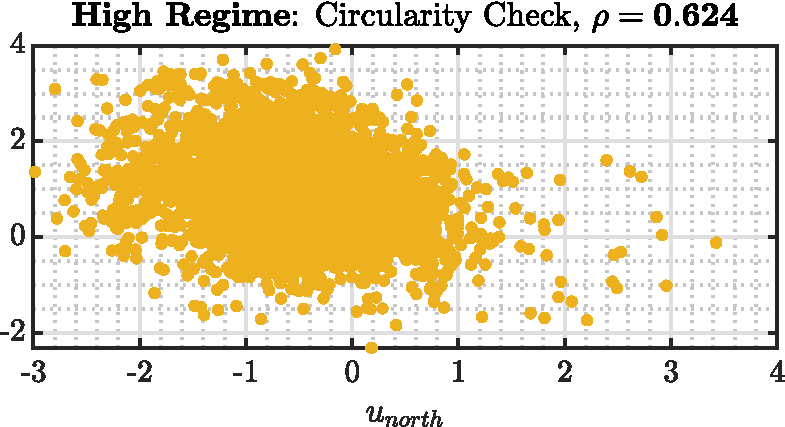
\includegraphics[height=1.5in]{report/widely-linear-filtering-and-adaptive-spectrum-estimation/complex-LMS-and-widely-linear-modelling/assets/b/circularity_3}
    \end{subfigure}
    ~
    \begin{subfigure}{0.49\textwidth}
        \centering
        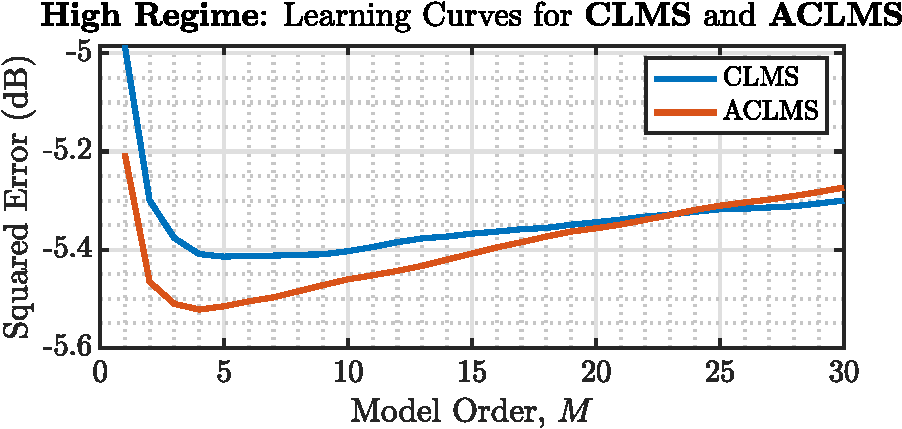
\includegraphics[height=1.5in]{report/widely-linear-filtering-and-adaptive-spectrum-estimation/complex-LMS-and-widely-linear-modelling/assets/b/learning_curves_3}
    \end{subfigure}
    \caption{High Regime:circularity plot and (A)CLMS learning curves.}
    \label{fig:4_1_b_3}
\end{figure}

%% c)
\item
%

Complex voltages are synthetically generated for various magnitude, angle combinations leading to balanced and unbalanced configurations, while their illustrations in the complex plane
are provided in figures \ref{fig:4_1_c_1}, \ref{fig:4_1_c_2}. Overall, we notice that balanced systems have a circular shape, while unbalanced don't.
This is also collaborated by the fact that the balanced system has circularity coefficient $\rho = 0$, while the unbalanced system has a high circularity coefficient, $\rho = 0.757$.
Finally, the impact of the angle and magnitude distortions, $\Delta_{b} \neq \Delta_{c} \neq 0$ and $V_{a} \neq V_{b} \neq V_{c}$, respectively, is depicted in figure \ref{fig:4_1_c_2}.

\begin{figure}[h]
    \centering
    \begin{subfigure}{0.49\textwidth}
        \centering
        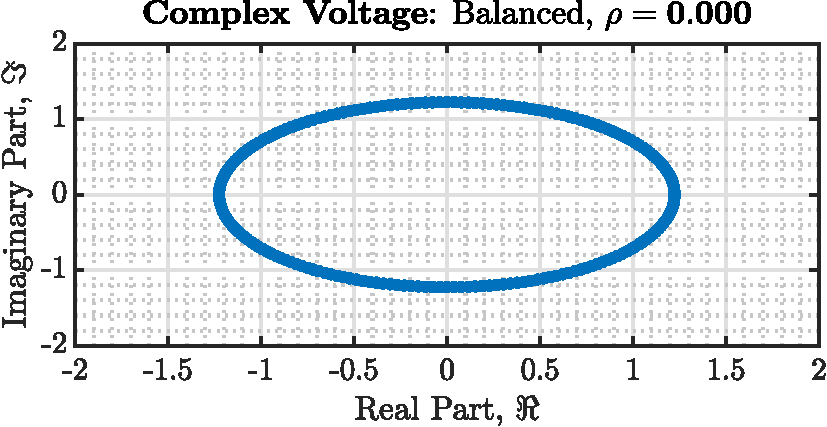
\includegraphics[height=1.5in]{report/widely-linear-filtering-and-adaptive-spectrum-estimation/complex-LMS-and-widely-linear-modelling/assets/c/balanced}
    \end{subfigure}
    ~
    \begin{subfigure}{0.49\textwidth}
        \centering
        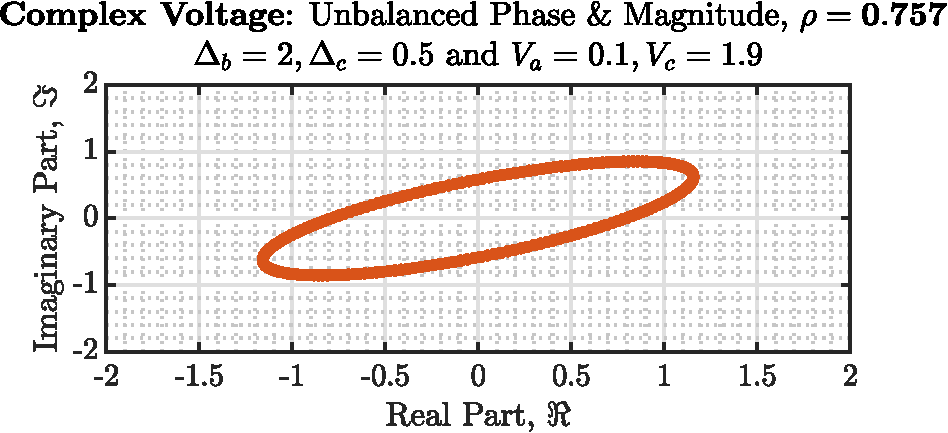
\includegraphics[height=1.5in]{report/widely-linear-filtering-and-adaptive-spectrum-estimation/complex-LMS-and-widely-linear-modelling/assets/c/unbalanced}
    \end{subfigure}
    \caption{Complex Voltage: balanced and unbalanced voltages.}
    \label{fig:4_1_c_1}
\end{figure}

\begin{figure}[h]
    \centering
    \begin{subfigure}{0.49\textwidth}
        \centering
        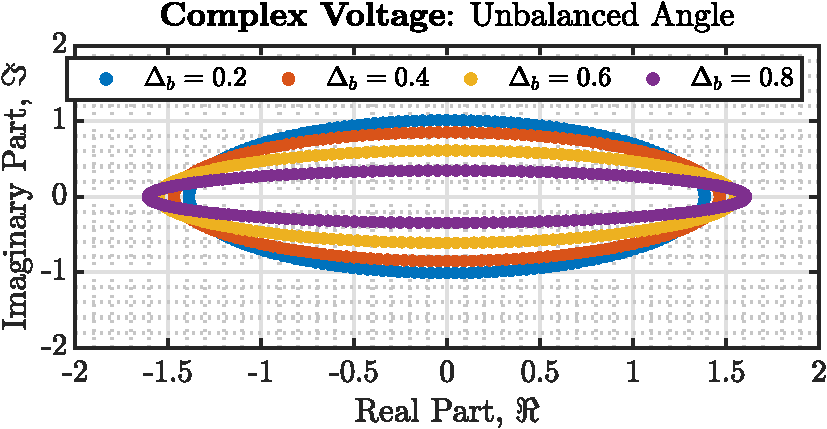
\includegraphics[height=1.5in]{report/widely-linear-filtering-and-adaptive-spectrum-estimation/complex-LMS-and-widely-linear-modelling/assets/c/unbalanced_angle}
    \end{subfigure}
    ~
    \begin{subfigure}{0.49\textwidth}
        \centering
        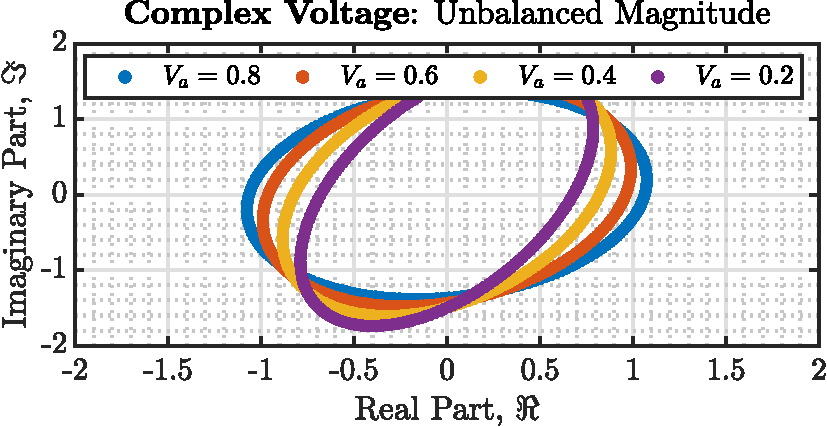
\includegraphics[height=1.5in]{report/widely-linear-filtering-and-adaptive-spectrum-estimation/complex-LMS-and-widely-linear-modelling/assets/c/unbalanced_magnitude}
    \end{subfigure}
    \caption{Complex Voltage: unbalanced voltages angle and magnitude distortions.}
    \label{fig:4_1_c_2}
\end{figure}

%% d)
\item
%

Balanced complex $\alpha\ -\ \beta$ voltages satisfy:

\begin{equation}
    u(n) = \sqrt{\frac{3}{2}} V e^{j(2\pi \frac{f_{o}}{f_{s}} n + \phi)}
\end{equation}

For time index $n+1$:

\begin{align}
    u(n+1)  &= \sqrt{\frac{3}{2}} V e^{j(2\pi \frac{f_{o}}{f_{s}} (n+1) + \phi)} \\
            &= \sqrt{\frac{3}{2}} V e^{j(2\pi \frac{f_{o}}{f_{s}} n + \phi)} e^{j 2 \pi \frac{f_{o}}{f_{s}}} \\
            &= u(n) e^{j 2 \pi \frac{f_{o}}{f_{s}}}
\label{eq:u_n+1}
\end{align}

Using the strictly linear autoregressive model of order 1, equation, satisfying:

\begin{equation}
    u(n+1) = u(n) h^{*}(n)
\end{equation}

we express the complex exponential in (\ref{eq:u_n+1}) as a function of the model parameter $h(n)$:

\begin{align}
    e^{j 2 \pi \frac{f_{o}}{f_{s}}} &= h^{*}(n) \\
    e^{-j 2 \pi \frac{f_{o}}{f_{s}}}&= h(n) \\
                                    &= | h(n) | e^{j\big( arctan \big(\frac{\Im\{h(n)\}}{\Re\{h(n)\}} \big) \big)}
\end{align}

Two complex numbers are equal if and only of both their magnitudes and their angles are equal, therefore we set the angles to be equal, obtaining:

\begin{align}
    2 \pi \frac{f_{o}}{f_{s}} = arctan \big(\frac{\Im\{h(n)\}}{\Re\{h(n)\}} \big) 
\end{align}

Solving for $f_{o}$ concludes the proof:

\begin{equation}
    f_{o} = \frac{f_{s}}{2\pi} arctan \big(\frac{\Im\{h(n)\}}{\Re\{h(n)\}} \big)
\label{proof:fo_CLMS}
\end{equation}

The unbalanced system satisfies:

\begin{equation}
    u(n) = A(n) e^{j(2\pi \frac{f_{o}}{f_{s}} n + \phi)} + B(n) e^{-j(2\pi \frac{f_{o}}{f_{s}} n + \phi)}
\label{eq:u_unbalanced}
\end{equation}

Using the widely linear autoregressive model of order 1, equation, satisfying:

\begin{equation}
    u(n+1) = h^{*}(n) u(n) + g^{*}(n) u^{*}(n)
\end{equation}

we substitute (\ref{eq:u_unbalanced}) terms:

\begin{align}
    u(n+1) =\ 
        &h^{*}(n) \bigg[ A(n) e^{j(2\pi \frac{f_{o}}{f_{s}} n + \phi)} + B(n) e^{-j(2\pi \frac{f_{o}}{f_{s}} n + \phi)} \bigg] + \nonumber\\
        &g^{*}(n) \bigg[ A^{*}(n) e^{-j(2\pi \frac{f_{o}}{f_{s}} n + \phi)} + B^{*}(n) e^{j(2\pi \frac{f_{o}}{f_{s}} n + \phi)} \bigg]
\label{eq:u_n+1_ar}
\end{align}

For time index $n+1$, the complex voltage satisfies:

\begin{equation}
    u(n+1) = A(n+1) e^{j(2\pi \frac{f_{o}}{f_{s}} (n+1) + \phi)} + B(n+1) e^{-j(2\pi \frac{f_{o}}{f_{s}} (n+1) + \phi)}
\label{eq:u_n+1_clarke}
\end{equation}

Equating (\ref{eq:u_n+1_ar}) and (\ref{eq:u_n+1_clarke}), collecting common exponential terms:

\begin{align}
    A(n+1) e^{j(2\pi \frac{f_{o}}{f_{s}} (n+1) + \phi)} &= \bigg[ h^{*}(n) A(n) + g^{*}(n) B^{*}(n) \bigg] e^{j(2\pi \frac{f_{o}}{f_{s}} n + \phi)} \\
    B(n+1) e^{-j(2\pi \frac{f_{o}}{f_{s}} (n+1) + \phi)} &= \bigg[ h^{*}(n) B(n) + g^{*}(n) A^{*}(n) \bigg] e^{-j(2\pi \frac{f_{o}}{f_{s}} n + \phi)}
\end{align}

Assuming that the amplitude change over time is negligible, or equivalently $A(n+1) \approx A(n)$ and $B(n+1) \approx B(n)$, the equations simplify as:

\begin{align}
    e^{j 2\pi \frac{f_{o}}{f_{s}}} = \frac{h^{*}(n) A(n) + g^{*}(n) B^{*}(n)}{A(n+1)} \approx h^{*}(n) + g^{*}(n) \frac{B^{*}(n)}{A(n)} \label{eq:e_A}\\
    e^{-j 2\pi \frac{f_{o}}{f_{s}}} = \frac{h^{*}(n) B(n) + g^{*}(n) A^{*}(n)}{B(n+1)} \approx h^{*}(n) + g^{*}(n) \frac{A^{*}(n)}{B(n)} \label{eq:e_B}
\end{align}

Note that (\ref{eq:e_A}) is the complex conjugate of (\ref{eq:e_B}, we reach:


\begin{align}
    h^{*}(n) + g^{*}(n) \frac{B^{*}(n)}{A(n)} = h(n) + g(n) \frac{A(n)}{B^{*}(n)}
\end{align}

Multiplying with $\frac{B^{*}(n)}{A(n)}$ both sides:

\begin{align}
    \bigg( h^{*}(n) - h(n) \bigg) \frac{B^{*}(n)}{A(n)} + g^{*}(n) \bigg( \frac{B^{*}(n)}{A(n)} \bigg)^{2} - g(n) = 0
\label{eq:quad}
\end{align}

We note that (\ref{eq:quad}) is quadratic in $\frac{B^{*}(n)}{A(n)}$, hence solving it we obtain:

\begin{align}
    \frac{B^{*}(n)}{A(n)}   &= \frac{- \bigg( h^{*}(n) - h(n) \bigg) \pm \sqrt{\bigg( h^{*}(n) - h(n) \bigg)^{2} + 4 g^{*}(n) g(n)}}{2g^{*}(n)} \\
                            &= \frac{2 \Im\{h(n)\}j \pm j\sqrt{-4 \Im\{h(n)\}^{2} + 4 |g(n)|^{2}}}{2g^{*}(n)} \\
                            &= \frac{\Im\{h(n)\}j \pm j\sqrt{\Im\{h(n)\}^{2} - |g(n)|^{2}}}{g^{*}(n)}
\end{align}

Substitution in (\ref{eq:e_A}), yields:

\begin{align}
    e^{j 2\pi \frac{f_{o}}{f_{s}}}  &= h^{*}(n) + \Im\{h(n)\}j \pm j\sqrt{\Im\{h(n)\}^{2} - |g(n)|^{2}} \\
                                    &= \Re\{h(n)\} \pm j\sqrt{\Im\{h(n)\}^{2} - |g(n)|^{2}} \\
\end{align}

Keeping one solution ($+$ sign), since $f_{s} \gg f_{o} > 0$:

\begin{align}
    e^{j 2\pi \frac{f_{o}}{f_{s}}}  &= \Re\{h(n)\} + j\sqrt{\Im\{h(n)\}^{2} - |g(n)|^{2}} \\
                                    &= \rho e^{j\big(\frac{\sqrt{\Im\{h(n)\}^{2} - |g(n)|^{2}}}{\Re\{h(n)\}}\big)}
\end{align}

where $\rho > 0$. Set the angles to be equal and solving for $f_{o}$ we complete the proof:

\begin{equation}
    f_{o} = \frac{f_{s}}{2 \pi} arctan \bigg(\frac{\sqrt{\Im\{h(n)\}^{2} - |g(n)|^{2}}}{\Re\{h(n)\}}\bigg)
\label{proof:fo_ACLMS}
\end{equation}

%% e)
\item
%

First order CLMS and ACLMS filters are trained on both the balanced and unbalanced (magnitude and angle) complex voltage synthetic data.
The derived formulae (\ref{proof:fo_CLMS}) and (\ref{proof:fo_ACLMS}) are used along with the learnt filter parameters, $h_{CLMS}$, $h_{ACLMS}$ \& $g_{ACLMS}$,
while the frequency estimates over time and the error curves are provided in figures \ref{fig:4_1_e_1}, \ref{fig:4_1_e_2} for the balanced and unbalanced complex voltage, respectively.

\begin{figure}[h]
    \centering
    \begin{subfigure}{0.49\textwidth}
        \centering
        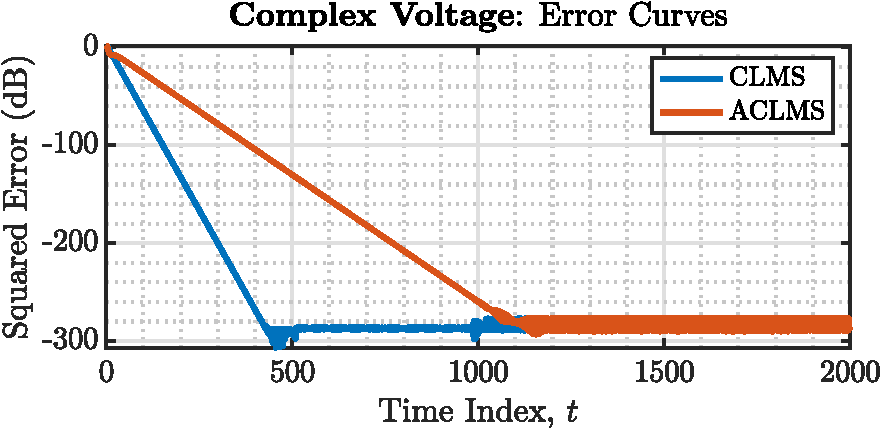
\includegraphics[height=1.5in]{report/widely-linear-filtering-and-adaptive-spectrum-estimation/complex-LMS-and-widely-linear-modelling/assets/e/balanced_error}
    \end{subfigure}
    ~
    \begin{subfigure}{0.49\textwidth}
        \centering
        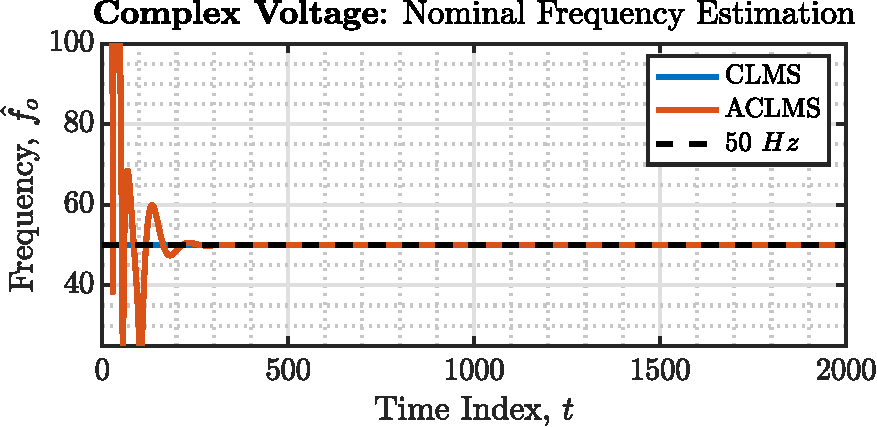
\includegraphics[height=1.5in]{report/widely-linear-filtering-and-adaptive-spectrum-estimation/complex-LMS-and-widely-linear-modelling/assets/e/balanced_frequency}
    \end{subfigure}
    \caption{Balanced Complex Voltage: mean squared prediction error (MPSE) and frequency estimation.}
    \label{fig:4_1_e_1}
\end{figure}

In case of the balanced grid, the CLMS filter excels, since it both converges faster to the nominal frequency $f_{o} = 50 Hz$, without overshooting (transient behaviour).
On the other hand, the ACLMS oscillates for the first $300$ timesteps and finally converges to the true frequency after that.
This is an expected result, since in figure \ref{fig:4_1_c_1} we showed that the balanced system has a circular complex voltage, which can be sufficiently modelled by a CLMS filter.
The extra degrees of ACLMS freedom, put a burden on the model, which needs more time to converge.

\begin{figure}[h]
    \centering
    \begin{subfigure}{0.49\textwidth}
        \centering
        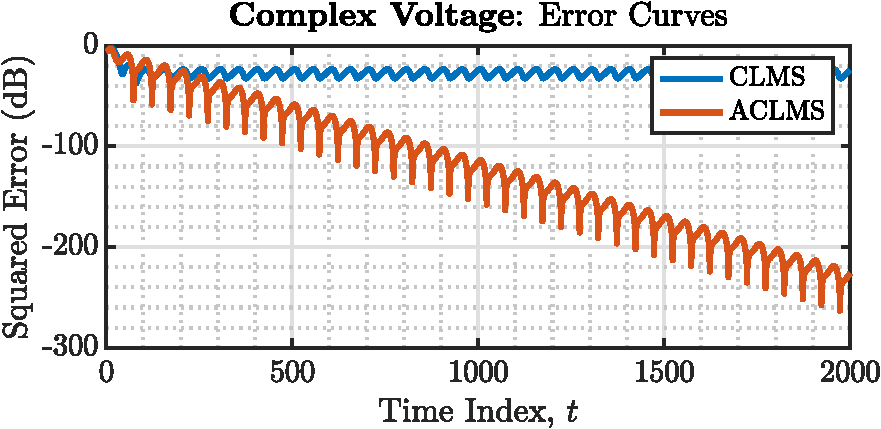
\includegraphics[height=1.5in]{report/widely-linear-filtering-and-adaptive-spectrum-estimation/complex-LMS-and-widely-linear-modelling/assets/e/unbalanced_error}
    \end{subfigure}
    ~
    \begin{subfigure}{0.49\textwidth}
        \centering
        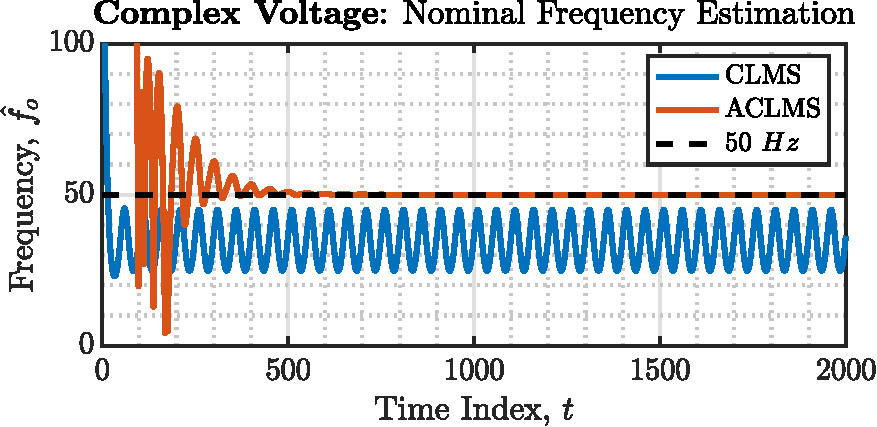
\includegraphics[height=1.5in]{report/widely-linear-filtering-and-adaptive-spectrum-estimation/complex-LMS-and-widely-linear-modelling/assets/e/unbalanced_frequency}
    \end{subfigure}
    \caption{Unbalanced Complex Voltage: mean squared prediction error (MPSE) and frequency estimation.}
    \label{fig:4_1_e_2}
\end{figure}

Figure \ref{fig:4_1_e_2} depicts the mean squared prediction error and frequency estimates for the unbalanced system,
with $(V_{a}, V_{b}, V_{c}) = (0.1, 1.0, 1.9)$ and $(\Delta_{b}, \Delta_{c}) = (2.0, 0.5)$.
In this scenario, the ACLMS converges to the true nominal frequency value after 450 timesteps, though the CLMS filter oscillates around $\hat{f}_{o} = 37 Hz$ and never adapts to the true $f_{o}$.
Unsurprisingly, CLMS does not have the capacity to model non-circular distributions and hence fails to model unbalanced configurations ($\rho = 0.757$).

%
\end{enumerate}